\chapter{Chapter 1 h1}

\section{What PolyTeX maps to in HTML}

  \texttt{texttt}: \kode{span.tt}

  \textsc{textsc}: \kode{span.sc}

  \textbf{textbf}

  \textit{textit}

  \underline{underline}

  \LaTeX\ LaTeX: a bunch of carefully styled spans

  Quote:

  \begin{quote}
  begin quote
  \end{quote}

  \subsection{Links}

    \kode|href|: \href{http://example.com}{Example domain.}

    TODO: \kode{url}? Using the package only works for PDF output.

    Markdown autolinks map to \kode{href} in PolyTeX.

    % \url{http://example.com}

  \subsection{Label}

    All labels becomes HTML IDs, and refs link to those IDs.

    \subsubsection{Label header}\label{label-header}

    \kode{ref} to this section~\ref{label-header}

      The tilde makes the descriptor \kode{section} become a single link with the \kode{ref}.

    \subsubsection{Cross file label}

      Label on another file: section~\ref{chapter-2}.

    \subsection{Header without label}

      Headers without labels cannot be referred to.

  \subsection{Figure}

    Small figure~\ref{fig-small}, large figure~\ref{fig-large}.

    \begin{figure}[htb]
      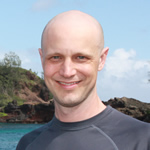
\includegraphics[width=2cm]{images/image.png}
      \caption{caption here}
      \label{fig-small}
    \end{figure}

    \begin{figure}[htb]
      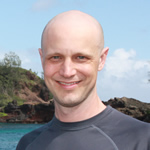
\includegraphics[width=5cm]{images/image.png}
      \caption{caption here}
      \label{fig-large}
    \end{figure}

    TODO how to center figures? If possible, without explicit center per figure environment?
    \kode{floatrow} package only works for the PDF output.

  \subsection{Table}

    Table reference: Table~\ref{table}.

    \begin{table}
      \caption{Table caption}
      \label{table}
      \begin{tabular}{|r|lc|}
          \hline
          a0    & a1 & a2 \\
          bbbb0 & b1 & b2 \\
          \hline
          \multicolumn{3}{|c|}{Multicolumn} \\
          \hline
        \end{tabular}
    \end{table}

  \subsection{Math}

  \begin{equation}
    \label{equation}
    x^2
  \end{equation}

  Inline only with \kode{\(  \)}, not dollar \kode{\$}: \( x^2 \) \$x\^{}2\$.

  Equation reference: Equation~\ref{equation}.

  \subsection{Code listing}

    TODO: how to escape brackets in kode?

    Inline with the custom \kode{kode} macro.

    Display with the custom \kode{code} environment.

    Code aligned relative to the begin.

    \begin{code}
    Put your code here.
    Put your code here.
    \end{code}
